% Supplementary body; compile Main.tex, which supplies the preamble and bibliography.

\section{A1. Brief Introduction to Baselines}

\noindent\textbf{DialogueRNN.}
This sequence-based ERC model~\cite{dialoguernn} uses
recurrent networks to track the global dialogue state, speaker states,
and emotion states. It explicitly accounts for speaker identity when
propagating conversational context.

\noindent\textbf{MMGCN.}
This method~\cite{mmgcn} constructs a multimodal fused graph and uses
graph convolution to capture multimodal dependencies together with
inter-speaker and intra-speaker contextual relations.

\noindent\textbf{MM-DFN.}
This model~\cite{mmdfn} introduces a graph-based dynamic fusion module
that captures contextual dynamics in different semantic spaces. Its
fusion process is designed to reduce redundant information and enhance
complementarity among modalities.

\noindent\textbf{M3Net.}
This approach~\cite{m3net} combines multivariate and multi-frequency
graph propagation to model multimodal conversational relations. The
multi-frequency branch captures emotion discrepancy and commonality at
different graph frequencies.

\noindent\textbf{Ada2I.}
This framework~\cite{ada2i} addresses modality imbalance through
Adaptive Feature Weighting and Adaptive Modality Weighting. These
modules perform feature-level and modality-level balancing by
leveraging intra-modal and inter-modal interactions.

\noindent\textbf{SDT.}
This model~\cite{sdt} combines intra-modal and inter-modal Transformer
encoders with gated multimodal fusion. It additionally uses unimodal
self-distillation to transfer supervision from the fused prediction
to the modality-specific branches.

\noindent\textbf{CSS.}
This framework~\cite{css} uses Synergistic Polynomial Fusion with
low-rank tensor composition to model higher-order multimodal
interactions. Its Pareto Gradient Modulator coordinates competing
learning objectives through Pareto-optimal update directions.

\section{A2. More Implementation Details}

\subsection{Input representations and context}
We use pre-extracted RoBERTa-large~\cite{liu2019roberta}, wav2vec
2.0~\cite{baevski2020wav2vec}, and DenseFace~\cite{zhao2018emotion}
representations for text, audio, and vision, respectively. Their input
dimensions are 1024, 1024, and 342. The textual representation of the
target utterance includes its preceding dialogue context, whereas the
acoustic and visual representations describe the target utterance. We
use the full dialogue history, up to 109 preceding utterances on
IEMOCAP and 32 on MELD.

\subsection{Architecture Details}
All modality features are projected to a common width of 256.
Modality-centric Cross-modal Alignment and learnable-query pooling use
eight attention heads. The Axis-wise Multimodal Mixer constructs six
learned elements per modality and uses two mixer blocks. Its
hidden-feature MLP has a hidden width of 1536. The Explicit Pairwise
Interaction Residual Correction uses an interaction rank of 32.

\subsection{Optimization Details}
We optimize MM-Mixer with AdamW. The learning rate is
$3\times10^{-5}$ on IEMOCAP and $4.17\times10^{-5}$ on MELD, with
weight decay values of $2\times10^{-4}$ and $9.98\times10^{-5}$,
respectively. The batch size is 32, and the maximum number of epochs
is 100 on IEMOCAP and 50 on MELD. The fusion dropout is 0.2 on both
datasets. We report the mean and standard deviation over three
independent runs.
The PolyLoss parameters are $\alpha_p=1.951$ and
$\gamma_p=1.402$, and the focal exponent is $\gamma_f=2.5$. On
IEMOCAP, the weights of the fused, textual, acoustic, and visual
objectives are 0.45, 0.33, 0.11, and 0.11. Its main objective uses
class weights and a detached batch-level focal coefficient shared by
all samples in a mini-batch. On MELD, the fused and three unimodal
objectives are equally weighted, and its unweighted main
classification loss uses differentiable sample-wise focal
coefficients. The auxiliary modality objectives use class-balanced
PolyLoss on both datasets.


\section{B1. Visualization Analysis}

\subsection{Component Ablations}
Figure~\ref{fig:supp_iemocap_ablation_tsne}
and Figure~\ref{fig:supp_meld_ablation_tsne} compare Full MM-Mixer with the
component-ablation variants using the same test utterances and t-SNE
settings. On IEMOCAP, the full model forms relatively compact regions
for sadness and anger. On MELD, joy and surprise also form recognizable
class-specific regions. Removing individual components alters these
local neighborhoods and weakens their organization, consistent with the
performance drops reported by the quantitative ablations in the main
paper.

\subsection{Comparison with Baselines}
Figure~\ref{fig:supp_model_tsne} compares the final fused
representations of the reproduced baselines and MM-Mixer on IEMOCAP
and MELD. Relative to several recurrent and graph-based baselines,
MM-Mixer exhibits more coherent class-wise organization. On IEMOCAP,
sadness and anger form compact and distinguishable regions, while on
MELD, joy and surprise show identifiable class-specific structures.
These qualitative patterns are consistent with the ACC and WF1
comparisons reported in the main paper.

\begin{figure*}[tp]
\centering
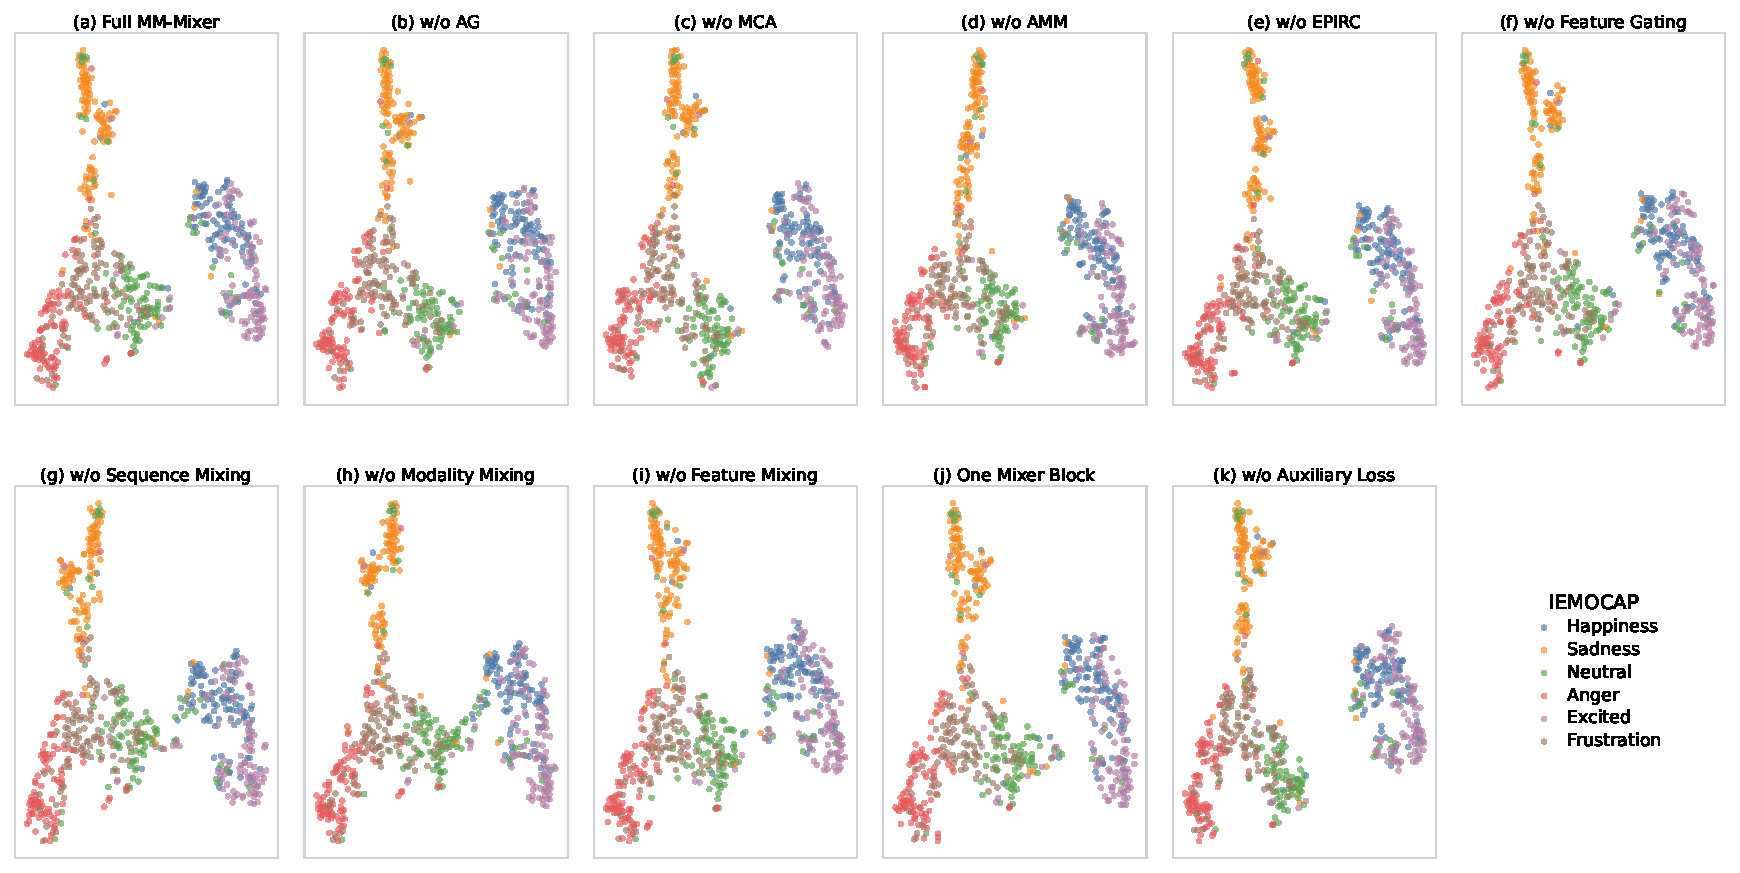
\includegraphics[width=\textwidth]
{iemocap-component-ablation-tsne-11panel.pdf}
\caption{Component-ablation t-SNE visualization on IEMOCAP. ``w/o''
denotes ``without.'' AG, MCA, AMM, and EPIRC denote Adaptive Gating,
Modality-centric Cross-modal Alignment, Axis-wise Multimodal Mixer,
and Explicit Pairwise Interaction Residual Correction, respectively.
``Sequence Mixing'' in the panels refers to mixing along the learned
projection axis, not observed temporal frames. Colors denote ground-truth
emotions.}
\label{fig:supp_iemocap_ablation_tsne}
\end{figure*}


\begin{figure*}[tp]
\centering
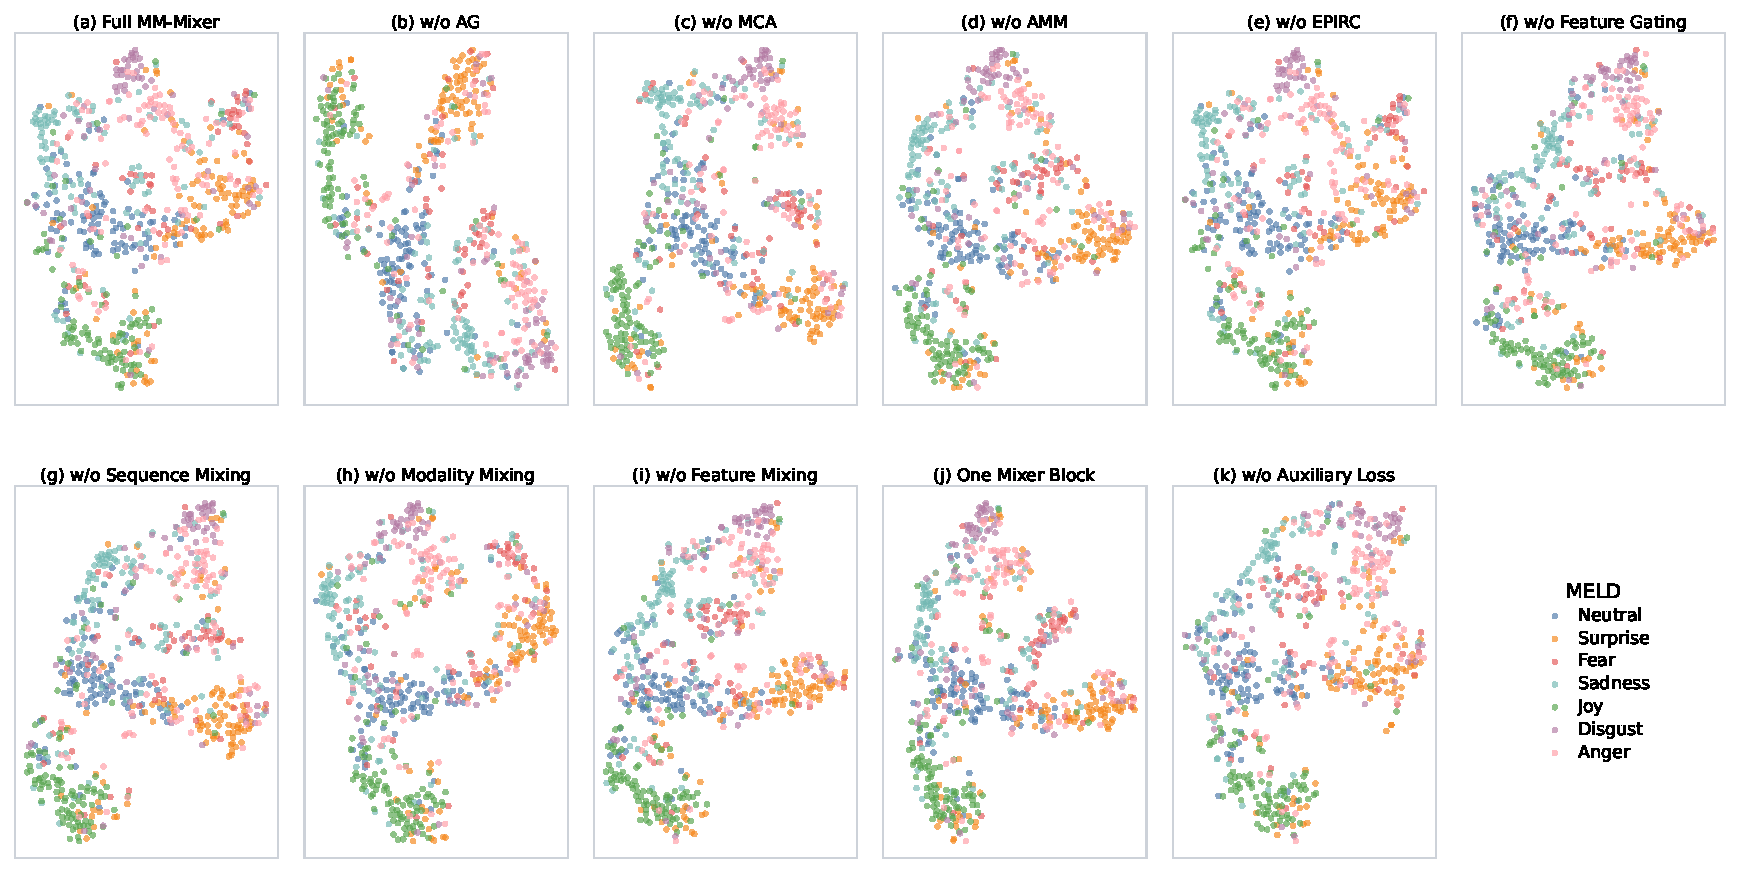
\includegraphics[width=\textwidth]
{meld-component-ablation-tsne-11panel.pdf}
\caption{Component-ablation t-SNE visualization on MELD. The variants,
sample-selection protocol, preprocessing, and abbreviations follow
Figure~\ref{fig:supp_iemocap_ablation_tsne}.}
\label{fig:supp_meld_ablation_tsne}
\end{figure*}

%\FloatBarrier
\begin{figure*}[tp]
\centering
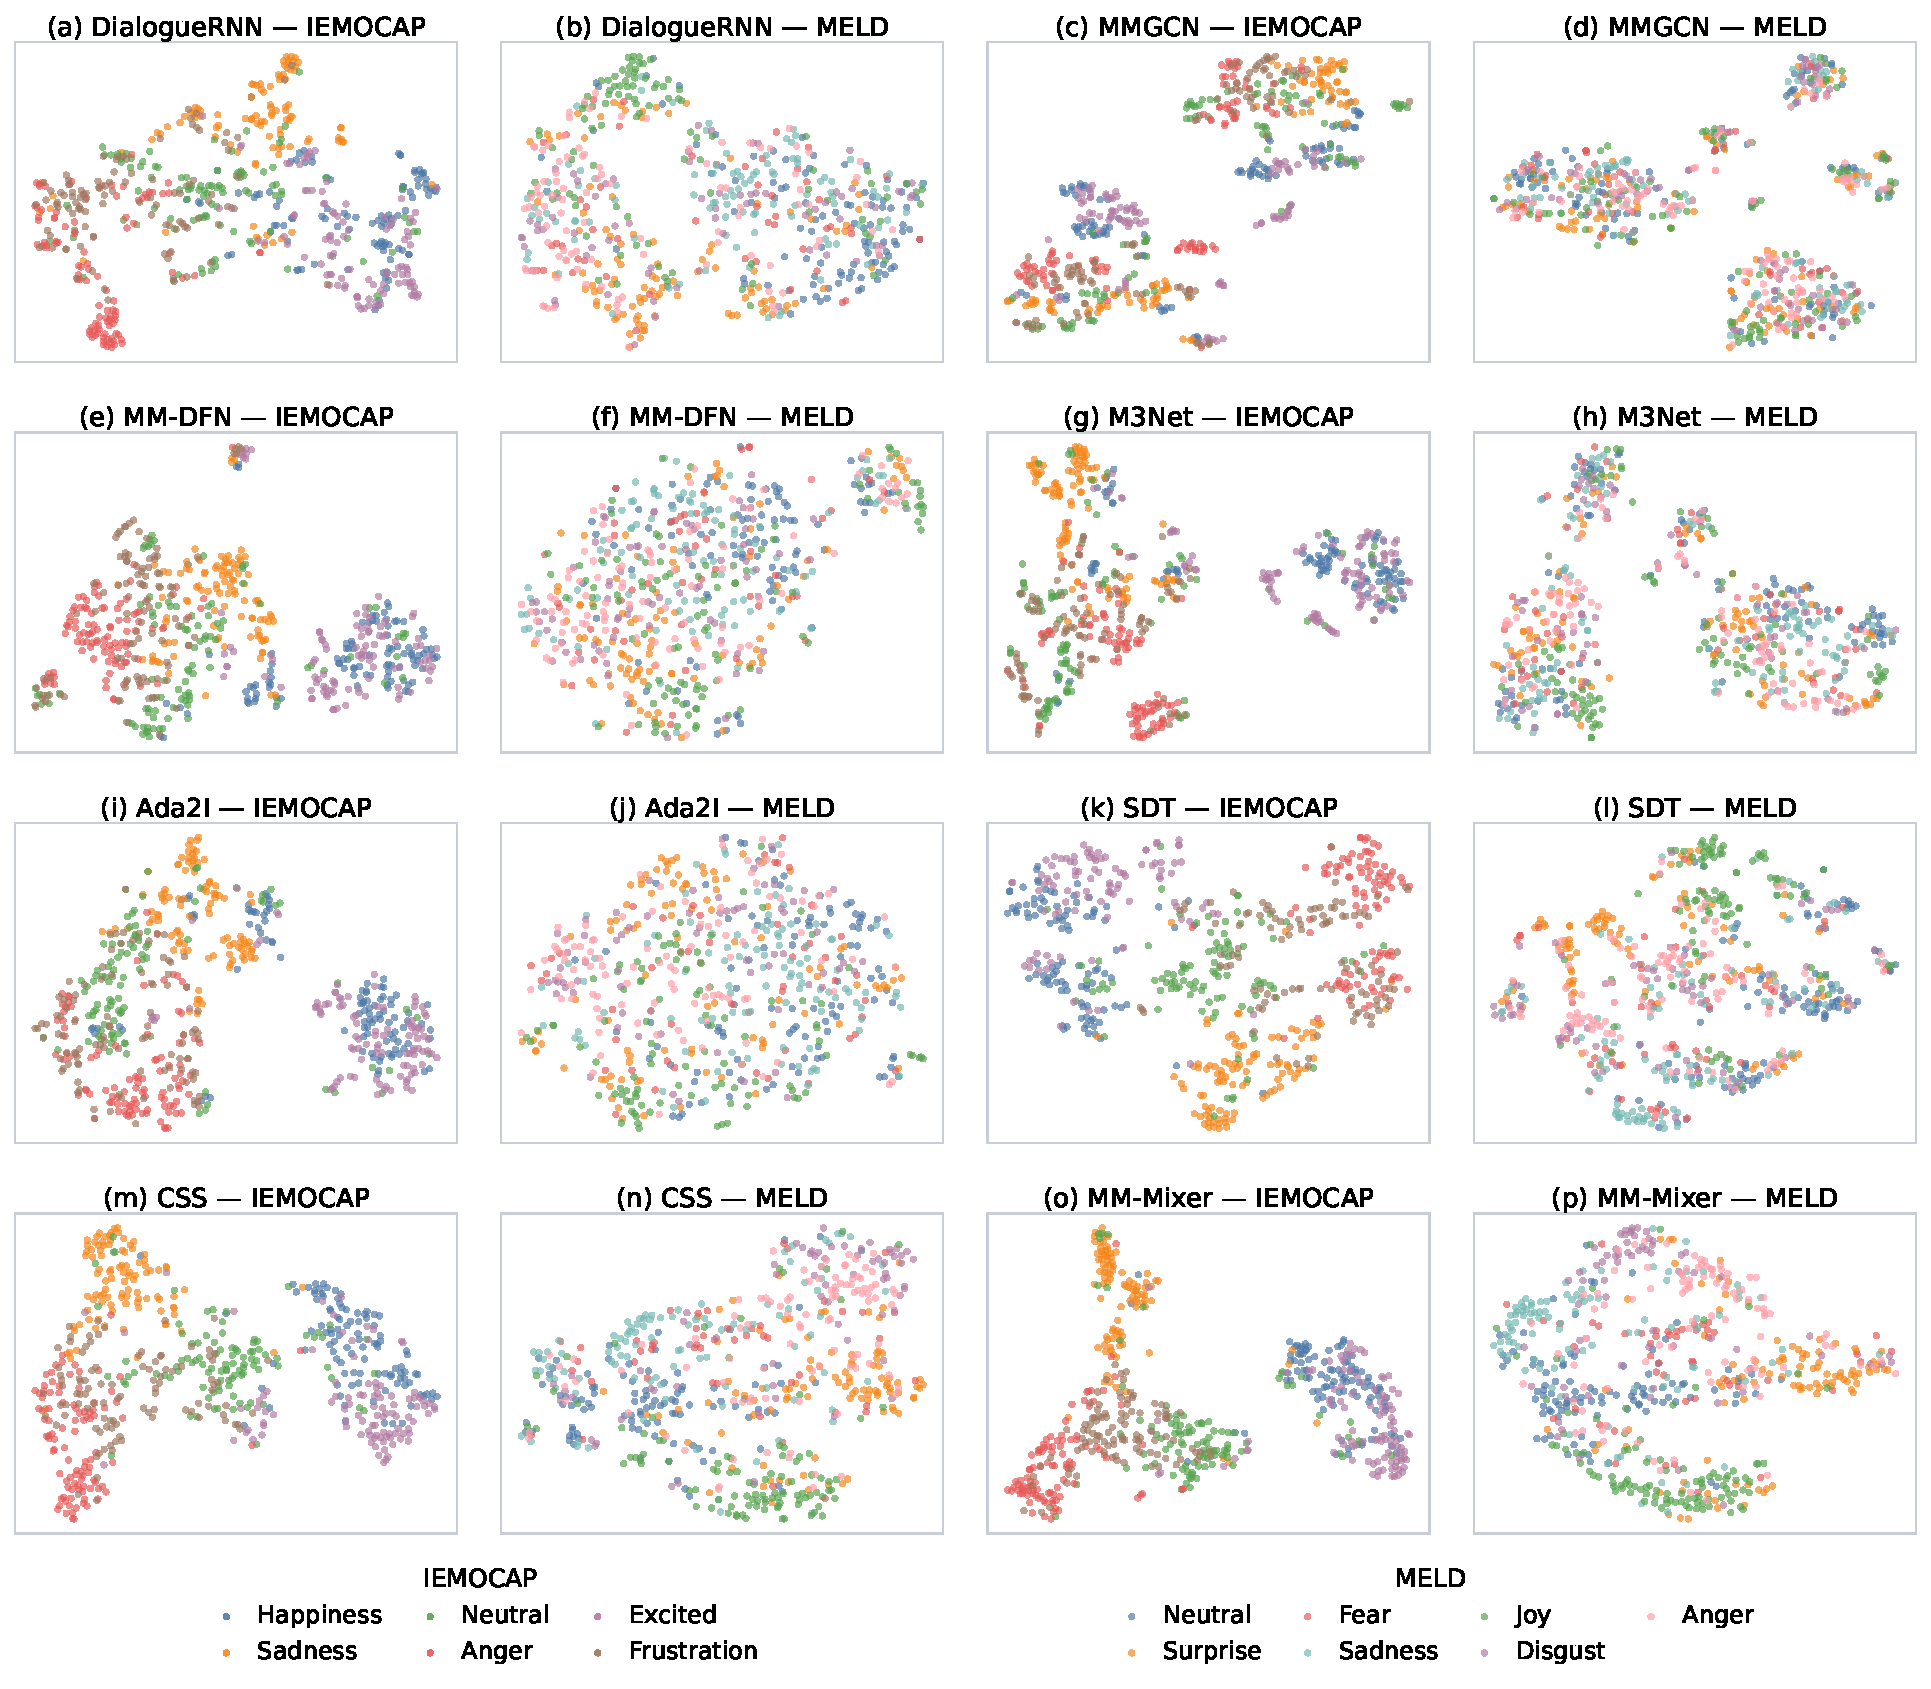
\includegraphics[width=\textwidth]
{model-comparison-tsne-16panel.pdf}
\caption{t-SNE visualization of the final fused representations
learned by eight models on IEMOCAP and MELD. For each model--dataset
pair, class-stratified test samples with the same per-class cap and
visualization settings are used. Colors denote ground-truth emotion labels.}
\label{fig:supp_model_tsne}
\end{figure*}
\FloatBarrier
